\chapter{Heuristic}
\section{Centroid}

The Centroid approach was used and implemented as a heuristic function in the project. As in, The heuristic function returns the average distance between the robot parts in the grid and the centroid point between them. As illustrated in figure \ref{fig:centroid_model}, every robot parts' X and Y coordinates are modeled as a point in the grid. The points are used to create a virtual polygon by the aid of the geometry library "JTS". The Centroid is calculated using Polygon.getCentroid() function from JTS library. Finally, the average distance between all points and the centroid is returned as the heuristic value.

\begin{figure}[H] 
   	\centering
	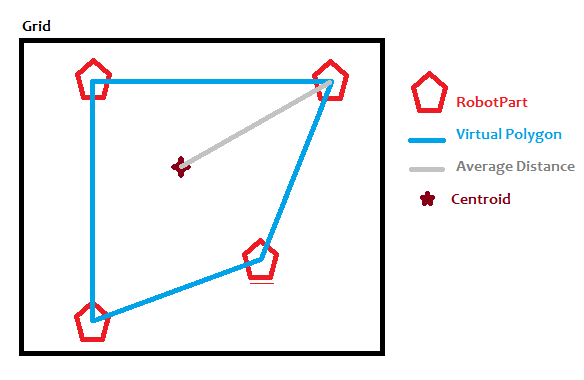
\includegraphics[scale=0.6]{images/Centroid} 
    \caption{Centroid concept illustration}
    \label{fig:centroid_model} 
\end{figure}

The heuristic approach proved to be a successful one, however it had a major drawback. If the Centroid can't be calculated because of the nature of the irregular shape e.g A twisted polygon as shown in figure \ref{fig:twistedcentroid}. The heuristic will return infinity. which wasn't acceptable. 

\begin{figure}[H] 
   	\centering
	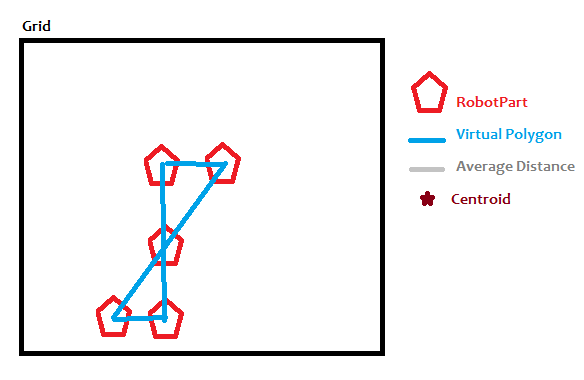
\includegraphics[scale=0.6]{images/twistedcentroid} 
    \caption{Centroid is incalculable incase of twisted polygons. }
    \label{fig:twistedcentroid} 
\end{figure}


\section{Average Distances}

Due to the Centroid unsuccessful attempt, the Average Distances approach was used. As in, it gets the summation of all the distances between all parts and each others as shown in figure \ref{fig:averagedistance}. The result is divided on the number of the parts Squared, to get an admissible Average Heuristic.

\begin{figure}[H] 
   	\centering
	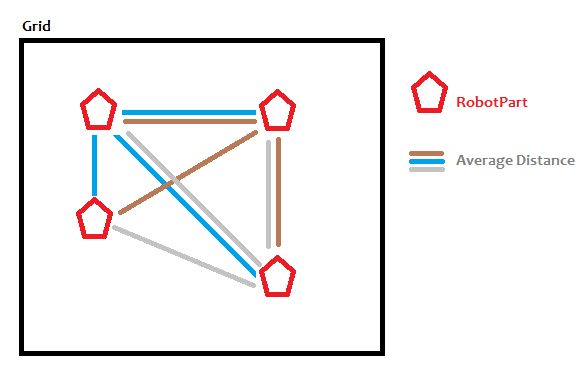
\includegraphics[scale=0.6]{images/averagedistance} 
    \caption{The distances between all parts and each other is used to evaluate the average distance. }
    \label{fig:averagedistance} 
\end{figure}

The heuristic approach is satisfying the \textbf{Centering} property. The heuristic function will check for merged up parts, returning a zero when all parts are conjoined, and returning the Average distance otherwise. \\

The approach followed is \textbf{consistent}. The heuristic value increases if one the parts stray away from the others, and decreases when it gains on other parts. The averaging is designed to get the Sum of distances and divide on the Number of parts squared. Thus, avoiding any chance for any overestimation of heuristic. Moreover, parts move in 2D grid, the average distance between 2 parts in a grid is the hypotenuse in most cases, which is always shorter than the catheti. and in case of straight lines, the distance is the same as the heuristic value (assuming distance is in unit steps), which proves \textbf{admissibility}.	


\section{Number of Bulks remaining}

The Number of Bulks remaining heuristic is a simple approach mainly used to assemble parts as fast as possible, The main concept is calculating the number of combined bulks of robot parts represented in the grid. Give more priority for small bulks to move, thus aiming to decrease the path cost by not moving the huge bulks to the smaller ones. Also, it gives more priority for parts merging into other parts, rather than stopping at an obstacle.  \\

The heuristic function is calculated as follows, the size of the bulks in the grid is doubled and added. Thus, bigger bulks will have larger output. The output is inversed to satisfy the \textbf{Monotonic} property by giving the bigger bulks less heuristic values. The function returns the number of parts in the board divided by the inversed value to satisfy the \textbf{admissibility} property. Finally, The \textbf{Centering} property is satisfied by a running check, returning a zero value if the number of bulks reaches one, i.e, there is only 1 merged robot. 